\section{为什么独立性需要乘积测度}
\label{sec:12-Real-Analysis-Support/06-Product-Measures-and-Fubini/01}

手上有两份日志。一份记录用户在推荐位上是否点击，一份记录同一次请求的加载延迟。各自的分布都好写。可只要开口问一句``延迟超过 300 毫秒、并且用户没有点击''的概率是多少，就得先有一个能同时容纳两条记录的样本空间；更麻烦的是，这个空间上的概率不能靠把两个边缘概率乘起来敷衍过去——两份日志之间可能有关联，而关联恰好藏在乘法失效的地方。

\subsection{联合问题要求一个新的样本空间}

给定两个可测空间 \((\Omega_1,\mathcal F_1)\) 与 \((\Omega_2,\mathcal F_2)\)，把结果成对地摆在一起，就得到乘积空间

\[
\Omega_1\times\Omega_2=\set{(\omega_1,\omega_2):\omega_1\in\Omega_1,\ \omega_2\in\Omega_2}.
\]

形如 \(A\times B\)（其中 \(A\in\mathcal F_1\)，\(B\in\mathcal F_2\)）的集合叫可测矩形，它对应``第一个分量落在 \(A\) 里、第二个分量落在 \(B\) 里''这一类问题。点击与延迟的联合事件正是这种形状。

但可问的问题远不止矩形。``延迟大于点击等待阈值的两倍''、``两个分量之差落在某区间''，这些集合在平面上是斜的、弯的，任何矩形都装不下。所以乘积 \(\sigma\)-代数

\[
\mathcal F_1\otimes\mathcal F_2\eqdef\sigma\bigl(\set{A\times B:A\in\mathcal F_1,\ B\in\mathcal F_2}\bigr)
\]

被定义为包含全体可测矩形的最小 \(\sigma\)-代数，它把矩形的并、交、补与可数极限一并封闭进来。关于 \(\sigma\)-代数为何要这样封闭，可参见\hyperref[sec:12-Real-Analysis-Support/05-Measure-Integration-and-Conditional-Expectation/01]{``\(\sigma\)-代数把可观察事件组织成封闭系统''}。两条实轴的乘积给出的正是 \(\R^2\) 上的 Borel \(\sigma\)-代数，二维的连续问题因此可以直接套用这套语言。

\subsection{矩形上的取值没有选择余地}

设 \((\Omega_1,\mathcal F_1,\mu)\) 与 \((\Omega_2,\mathcal F_2,\nu)\) 是两个测度空间。若要把``两个分量彼此不施加影响''翻译成一个测度，那么在矩形上它只能取一个值：

\[
(\mu\times\nu)(A\times B)=\mu(A)\,\nu(B).
\]

这一步几乎不需要论证——面积等于长乘宽，概率等于两个概率相乘，都是同一个式子。困难在下一步：\(\mathcal F_1\otimes\mathcal F_2\) 里绝大多数集合不是矩形，甚至不是可数个矩形的并，上面那条规则对它们只字未提。

\begin{center}
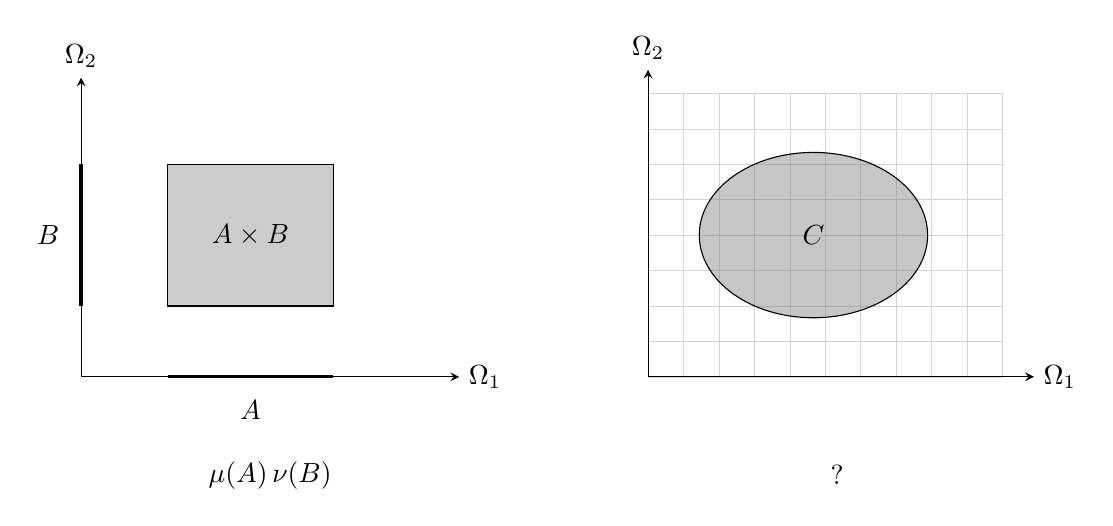
\begin{tikzpicture}[>=stealth]
% 左panel：矩形，取值被锁死
\draw[->] (0,0) -- (4.8,0) node[right] {\(\Omega_1\)};
\draw[->] (0,0) -- (0,3.8) node[above] {\(\Omega_2\)};
\fill[gray,opacity=0.40] (1.1,0.9) rectangle (3.2,2.7);
\draw (1.1,0.9) rectangle (3.2,2.7);
\draw[very thick] (1.1,0) -- (3.2,0);
\draw[very thick] (0,0.9) -- (0,2.7);
\node at (2.15,-0.42) {\(A\)};
\node at (-0.42,1.8) {\(B\)};
\node at (2.15,1.8) {\(A\times B\)};
\node at (2.4,-1.25) {\(\mu(A)\,\nu(B)\)};
% 右panel：一般事件，取值需要延拓
\begin{scope}[shift={(7.2,0)}]
\draw[step=0.45,gray!35,very thin] (0,0) grid (4.5,3.6);
\draw[->] (0,0) -- (4.9,0) node[right] {\(\Omega_1\)};
\draw[->] (0,0) -- (0,3.9) node[above] {\(\Omega_2\)};
\fill[gray,opacity=0.45] (2.1,1.8) ellipse (1.45 and 1.05);
\draw (2.1,1.8) ellipse (1.45 and 1.05);
\node at (2.1,1.8) {\(C\)};
\node at (2.4,-1.25) {\(?\)};
\end{scope}
\end{tikzpicture}
\end{center}

\emph{左边矩形上的值被两个边缘测度锁死，右边这种一般事件只能靠可数个矩形去围，值必须由延拓定理指定。}

\subsection{可数可加性在乘积空间上不是白送的}

把矩形的有限不交并收集起来，得到一个代数 \(\mathcal A\)；在 \(\mathcal A\) 上用``拆成矩形、逐块相乘再相加''来定义集函数，有限可加性容易验证。要调用 Carath\'eodory 扩张定理，还差一步：这个集函数在 \(\mathcal A\) 上必须是可数可加的。也就是说，若一个矩形被可数个互不相交的矩形铺满，

\[
A\times B=\bigsqcup_{n\ge 1}A_n\times B_n,
\]

就必须有 \(\mu(A)\nu(B)=\sum_{n\ge1}\mu(A_n)\nu(B_n)\)。这条等式不是记号上的自动结论，它要靠积分来证。把上式两边写成指示函数并固定第一个坐标 \(x\)，得到

\[
\ind_A(x)\,\nu(B)=\sum_{n\ge1}\ind_{A_n}(x)\,\nu(B_n),
\]

这是因为对固定的 \(x\)，两边都在计算同一个截口的 \(\nu\)-测度。再对 \(x\) 关于 \(\mu\) 积分，用单调收敛定理把求和号搬到积分号外，就得到所要的等式。用到的工具正是\hyperref[sec:12-Real-Analysis-Support/04-Limits-and-Integration/02]{``控制收敛用一个可积包络守住质量''}那一路的极限交换手段。

条件对账：单调收敛只要求被积项非负，这里全是测度值，自动满足；而扩张的唯一性另需 \(\mu\) 与 \(\nu\) 都是 \(\sigma\)-有限的，即全空间可以被可数个有限测度集覆盖。长度、计数、概率测度都满足这一条。若丢掉 \(\sigma\)-有限性，可以造出两个不同的测度在所有矩形上一致、在某个一般集合上分道扬镳——图中右边那个问号，此时确实答不上来。

延拓得到的测度 \(\mu\times\nu\) 称为乘积测度。两枚公平骰子的联合分布，36 个结果各占 \(1/36\)，正是两个``六点各 \(1/6\)''的测度的乘积。

\begin{definition}[乘积测度]
设 \((\Omega_1,\mathcal F_1,\mu)\) 与 \((\Omega_2,\mathcal F_2,\nu)\) 为 \(\sigma\)-有限测度空间。存在唯一的测度 \(\mu\times\nu\) 定义在 \(\mathcal F_1\otimes\mathcal F_2\) 上，使得对一切 \(A\in\mathcal F_1,\ B\in\mathcal F_2\) 有 \((\mu\times\nu)(A\times B)=\mu(A)\nu(B)\)。
\end{definition}

\subsection{独立就是联合测度等于乘积测度}

设 \(X,Y\) 是同一概率空间上的随机变量。它们的联合分布是乘积空间上的测度 \(P_{X,Y}(C)=P\bigl((X,Y)\in C\bigr)\)，边缘分布 \(P_X,P_Y\) 由投影到两个坐标得到。有了乘积测度，独立性可以写成一句不含密度、不含条件概率的等式：

\[
X\perp Y
\quad\Longleftrightarrow\quad
P_{X,Y}=P_X\times P_Y .
\]

限制到矩形上，它退回熟悉的 \(P(X\in A,\ Y\in B)=P(X\in A)\,P(Y\in B)\)。两种写法等价，因为矩形生成整个乘积 \(\sigma\)-代数，而两个测度若在一个生成 \(\pi\) 系上一致（矩形对交封闭，正是 \(\pi\) 系），在生成的 \(\sigma\)-代数上就处处一致。测度写法的好处是它一次性覆盖了图中右边那种弯曲的、斜的事件：独立性对它们同样给出因式分解，而不只对方方正正的矩形有效。

由此还能立刻读出一条封闭性：若 \(X\perp Y\)，则对任意可测函数 \(g,h\)，仍有 \(g(X)\perp h(Y)\)。理由是 \(g(X)\) 生成的事件都属于 \(X\) 生成的 \(\sigma\)-代数，因式分解沿着包含关系传递下去。平方、取符号、按阈值二值化，都不会把独立弄成相关。

\subsection{边缘分布记不住关联}

回到开头的两份日志。假设点击率是 \(0.1\)，延迟超过 300 毫秒的比例是 \(0.2\)。这两个数字无论怎么摆弄，都推不出联合概率 \(P(\text{未点击},\ \text{延迟高})\)——它可以是独立情形下的 \(0.9\times0.2=0.18\)，也可以更大，如果慢请求确实劝退了用户。关联既不在第一个边缘里，也不在第二个边缘里，它只住在联合测度与乘积测度的差里。

这解释了一个常见的建模顺序：先写联合分布，再谈边缘与条件，而不是反过来。\hyperref[sec:05-Probability/05-Joint-Distributions/01]{``联合、边缘与条件分布''}一篇在离散与连续的语言下讲过同一件事，这里只是把它说得更严格一层：边缘是投影，投影会丢信息，而丢掉的那部分正是我们最关心的依赖结构。

多于两个空间时，乘积按结合律逐步搭起来：\((\mu_1\times\mu_2)\times\mu_3\) 与 \(\mu_1\times(\mu_2\times\mu_3)\) 在自然对应下是同一个测度。独立同分布样本的联合分布就是同一概率测度的 \(n\) 重乘积，机器学习里那句``训练集独立同分布''的假设，写成测度语言正是这个乘积。无穷多个因子时还要 Kolmogorov 延拓定理来保证极限对象存在，那是随机过程的地基，本单元不涉及。

乘积测度既然造好了，下一个问题就摆在面前：在乘积空间上算积分时，能不能先积一个变量再积另一个？下一节给出两条定理和它们各自的门槛。
